\section{Experimental Setup}
\subsection{Mass Modelling and Regimes}
Lets model an exponential disk using these rings. The mass density \( \rho \) in an exponential disk decays exponentially with
radius
\begin{equation}
    \rho(R) = \rho_0 \exp\left(-\frac{R}{R_d}\right) \label{eq:exponential_disk_density}
\end{equation}
where \( R_d \) is the disk scale length and \( \rho_0 \) is the scale density. We can then calculate the ring's total mass
as the mass density integrated over the ring's perimeter but to simplify we will instead integrate over a circle whose radius is
given by the ring's scale radius \( R \).
Hence the mass of a ring is simply the circumference \( 2\pi R \) multiplied by the mass density \( \rho(R) \) which gives
\begin{equation}
    M(R) = \frac{M_{d}R}{R_d} \exp\left(-\frac{R}{R_d}\right)\label{eq:ring_mass}
\end{equation}
where \( M(R) \) is the ring mass, \( R \) is the radial distance from the origin, \( M_{d} \) is the mass scale of the disk and
\( r_{d} \) is the scale length of the disk. Note that we have subsumed \( 2\pi \) into \( M_0 \). The stationary points are
given by \( \dbyd{M}{R} = 0 \)
\begin{align}
    \dbyd{M}{R} & = \frac{M_{d}}{R_d} \exp\left(-\frac{R}{R_d}\right) - \frac{M_{d}R}{R_d^2} \exp\left(-\frac{R}{R_d}\right) \nonumber \\
                & = \frac{M_{d}}{R_d} \exp\left(-\frac{R}{R_d}\right)\left(1 - \frac{R}{R_d}\right) \nonumber                          \\
    0           & = \frac{M_{d}}{R_d} \exp\left(-\frac{R}{R_d}\right)\left(1 - \frac{R}{R_d}\right) \nonumber                          \\
    \implies R  & = R_{d}
\end{align}
Considering its plot as seen in Fig.~\ref{fig:ring_mass}, this point is a maximum.

\begin{figure}
    \begin{center}
        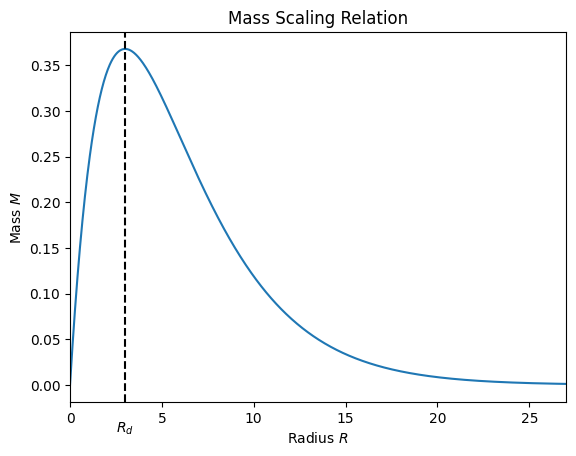
\includegraphics[width=0.8\textwidth]{resources/ring_mass_scaling.png}
        \caption{The mass scaling function from \( R = 0 \) to \( R=27 \) with \( M_d = 1 \) and \( R_d = 3 \).}\label{fig:ring_mass}
    \end{center}
\end{figure}

We now want to explore how this mass scaling affects the scaling of the inertia tensor components to see if there are different
regimes.

\subsection{Inertia Tensor Components Scaling Relations}
Recall that the inertia tensor components are
\begin{align*}
    I_{xx} & = M
    \left[
        \frac{K\left(-{e'}^{2}\right) -\left(1 - e^2\right)E\left(-{e'}^{2}\right)}{e^2K\left(e^2\right)}
        \right]
    ab R^2                                                           \\
    I_{yy} & = M
    \left[
        \frac{E\left(-{e'}^{2}\right) - K\left(-{e'}^{2}\right)}{e^2K\left(e^2\right)}
        \right]
    ab R^2                                                           \\
    I_{zz} & = M \frac{E\left(e^2\right)}{K\left(e^2\right)} a^2 R^2
\end{align*}
and notice that the components are proportional to the quantity
\begin{equation}
    I_{\alpha\alpha} \propto M(R)R^2 \label{eq:inertia_mass_radius_scaling}
\end{equation}
where \( \alpha \in \left\{ x, y, z \right\} \), as we have imposed that the mass is a function of radius, but the %chktex 21
other terms such as the eccentricity and semi-minor and major axes scale lengths are constant. Substituting
Eqn.~\ref{eq:ring_mass} into Eqn.~\ref{eq:inertia_mass_radius_scaling} gives us the pure radius scaling relation of the inertia
tensor components
\begin{align}
    I_{\alpha\alpha}          & \propto \frac{M_{d}R}{R_d} \exp\left(-\frac{R}{R_d}\right) R^2 \nonumber      \\
                              & \propto \frac{M_{d}R^3}{R_d} \exp\left(-\frac{R}{R_d}\right) \nonumber        \\
    \implies I_{\alpha\alpha} & \propto R^3 \exp\left(-\frac{R}{R_d}\right) \label{eq:inertia_radius_scaling}
\end{align}
Differentiating this with respect to \( R \) gives us the stationary points of the scaling relation,
\begin{equation}
    \dbyd{I_{\alpha\alpha}}{R}= C\left[3R^2 \exp\left(-\frac{R}{R_d}\right) - \frac{R^3}{R_d} \exp\left(-\frac{R}{R_d}\right)\right]
\end{equation}
where \( C \) is the proportionality constant. Setting this to zero and solving for \( R \) gives us the stationary points
\begin{align}
    0             & = C\left[3R^2 \exp\left(-\frac{R}{R_d}\right) - \frac{R^3}{R_d} \exp\left(-\frac{R}{R_d}\right)\right] \nonumber \\
                  & = 3R^2 - \frac{R^3}{R_d} \nonumber                                                                               \\
                  & = 3 - \frac{R}{R_d} \nonumber                                                                                    \\
    \frac{R}{R_d} & = 3 \nonumber                                                                                                    \\
    \implies R    & = 3R_d
\end{align}
hence there is a stationary point at \( R = 3R_d \). The second derivative of the inertia tensor components will then help
determine whether this point is a maximum, minimum or a saddle point.
% NOTE: Not bothered to write the derivation of the second derivative
\begin{equation}
    \frac{d^2I_{\alpha\alpha}}{dR^2} = CR\frac{6R_d^2 - 6R_d R + R^2}{R_d^2} \exp\left(-R/R_d\right)
\end{equation}
Evaluating at \( R = 3R_d \) gives the value
\begin{equation}
    \frac{d^2I_{\alpha\alpha}}{dR^2} = -9CR_d\exp(-3) < 0
\end{equation}
and so the point \( R=3R_d \) is a maximum. This is clear when looking at its plot in Fig.~\ref{fig:inertia_radius_scaling}.

\begin{figure}
    \begin{center}
        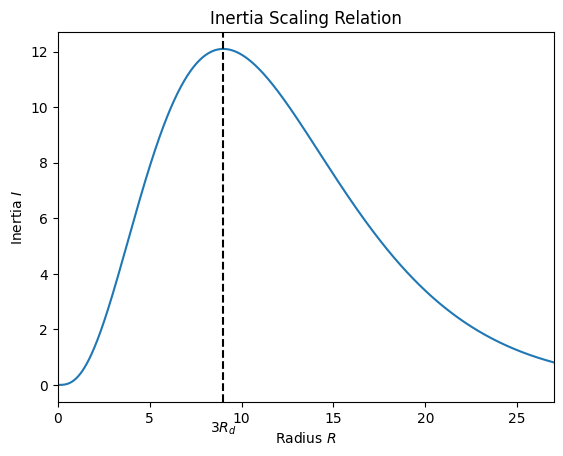
\includegraphics[width=0.8\textwidth]{resources/ring_inertia_scaling.png}
        \caption{The inertia tensor components scaling function from \( R = 0 \) to \( R=27 \) with \( M_d = 1 \) and \( R_d = 3 \).}\label{fig:inertia_radius_scaling}
    \end{center}
\end{figure}

\subsection{Regimes}
Therefore there are three regimes to consider
\begin{enumerate}
    \item{
                \( R < R_d \): The mass and inertia tensor components are both increasing with radius.
          }
    \item{
                \( R_d < R < 3R_d \): The mass is decreasing with radius but the inertia tensor components are increasing.
          }
    \item{
                \( R > 3R_d \): The mass and inertia tensor components are both decreasing with radius.
          }
\end{enumerate}
Hence we will run simulations for these three regimes. An issue to consider when setting the disk scale length parameter \( R_d \)
is the problem of rings bunching up together. If the rings are separated by a small amount in radius, there can be regions
where the density is very large which causes extreme torques. This leads to numerical instability with the current scheme and
so to limit the effect we must use a large disk scale length.